\documentclass[EEEE]{KGCOEReport}

\usepackage[backend=biber]{biblatex}
\usepackage{graphicx}
\usepackage{newtxtext, newtxmath}
\usepackage{csquotes}
\usepackage{parskip}
\usepackage{karnaugh-map}
\usepackage{amsmath}
\usepackage{circuitikz}
\usepackage{hyperref}
\usepackage{float}
\usepackage{pdfpages}

\graphicspath{./assets/}
\addbibresource{./assets/bib.bib}

\newcommand{\classCode}{EEEE 281}
\newcommand{\className}{Circuits 1}

\newcommand{\name}{Aden Perry}
% \newcommand{\partnerName}{PARTNER}

\newcommand{\LabSectionNum}{L7}

\newcommand{\TAs}{Sol Holston}
\newcommand{\exerciseNumber}{2}
\newcommand{\exerciseDescription}{Nodal Analysis}

\newcommand{\dateDone}{2026-02-24}
\newcommand{\dateSubmitted}{2026-03-03}


\begin{document}

\maketitle

\section*{Abstract}

The purpose of this exercise was to analyze a transistor circuit and determine
the voltages of each terminal relative to a ground, as well as the voltage from
the base to the emitter. The nodal analysis technique was applied. The circuit
was simulated using LTspice. A DC Bias point simulation was conducted. The
simulated values were used to verify the voltages calculated by hand. The
circuit was implemented in hardware. It was stimulated using two 5 volt sources
applied. One source was applied from a terminal of the circuit to a ground. The
other source was applied from the ground to the other terminal of the circuit,
such that there was a 10 volt difference in potential across the two terminals.
The voltages across the transistor were measured using a digital mulitmeter.
The measured values were very close to the calculated and simulated values; the
exercise was successful.

\section{Introduction and Theory}

The objective of this laboratory was to calculate the voltages from transistor
terminals to ground using nodal analysis; to implement a transistor circuit in
hardware; and to measure and verify the voltages.

\subsection{Theory: Circuit Investigated}

A transistor circuit is given in Figure \ref{fig:c1}.

\begin{figure}[H]
	\center
	\includegraphics[width=0.5\textwidth]{figures/circuit-1.pdf}
	\caption{Transistor Circuit}
	\label{fig:c1}
\end{figure}

The circuit has two voltage sources and a number of resistors. By inspection,
node $v_1 = 5$ volts and node $v_2 = -5$ volts. The node equation for node
$v_b$ is trivial. By inspection, $v_e = v_b - 0.7$. By inspection, the sum of
currents leaving the collector node and the currents leaving the emitter node
are equal to 17 microamps. This system of equations can be solved using Cramer's
rule, a matrix for which is given in Equation \ref{equ:e1}.

\begin{equation}
	\begin{bmatrix}
		1           & 0                    & 0                   & 0        & 0                 \\
		0           & 1                    & 0                   & 0        & 0                 \\
		-4,700^{-1} & -2,200^{-1}          & 6.673 \cdot 10^{-4} & 0        & 0                 \\
		0           & 0                    & -1                  & 1        & 0                 \\
		-1,000^{-1} & -2.228 \cdot 10^{-3} & 0                   & 470^{-1} & 1.1 \cdot 10^{-3}
	\end{bmatrix}
	\cdot
	\begin{bmatrix}
		v_1 \\ v_2 \\ v_b \\ v_e \\ v_c
	\end{bmatrix}
	=
	\begin{bmatrix}
		5 \\ -5 \\ -17 \cdot 10^{-6} \\ -0.7 \\ 17 \cdot 10^{-6}
	\end{bmatrix}
	\label{equ:e1}
\end{equation}

Thus,

\begin{align}
	v_c                             & = \fbox{$-0.657525 \text{ V}$} \\
	v_b                             & = \fbox{$-1.83707 \text{ V}$}  \\
	v_e                             & = \fbox{$-2.53707 \text{ V}$}  \\
	v_{be}  = -1.83707 - (-2.53707) & = \fbox{0.7 V}
\end{align}

\subsection{Theory: LTspice Simulation}

The transistor circuit given in Figure \ref{fig:c1} was simulated in LTspice.
The schematic is shown in Figure \ref{fig:lts}.

\begin{figure}[H]
	\center
	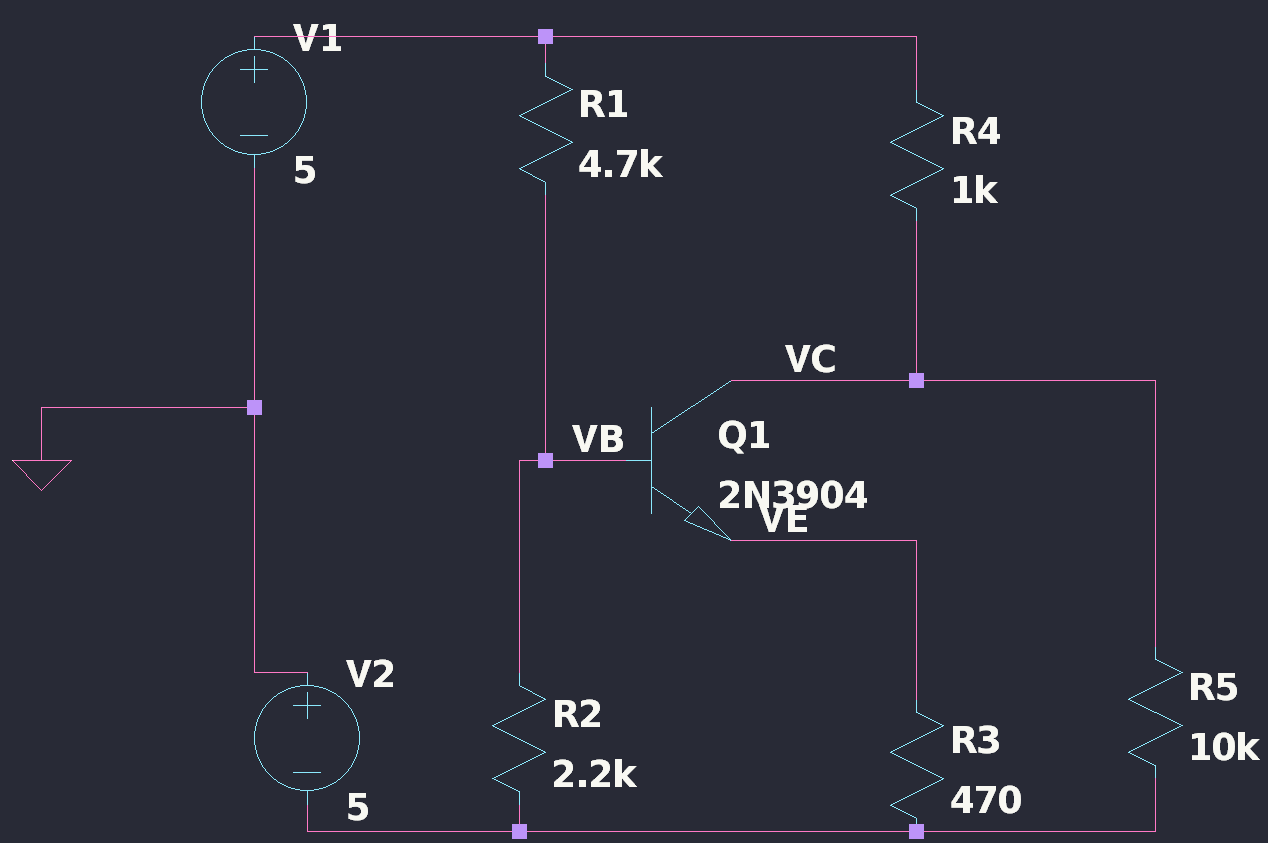
\includegraphics[width=0.5\textwidth]{assets/c1-lts.png}
	\caption{Transistor Circuit in LTspice}
	\label{fig:lts}
\end{figure}

The LTspice given in Figure \ref{fig:lts} was used to run a DC bias point
simulation. The simulation results are given in Figure \ref{fig:lts-res}.

\begin{figure}[H]
	\center
	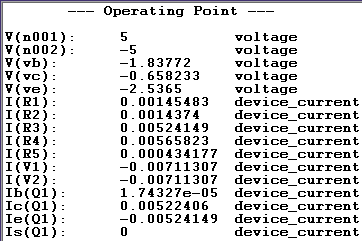
\includegraphics[width=0.5\textwidth]{assets/c1-lts-val.png }
	\caption{Transistor Circuit in LTspice Simulation Results}
	\label{fig:lts-res}
\end{figure}

The results given in Figure \ref{fig:lts-res} show simulated voltages
$v_c = -0.658$, $v_b = -1.838$, and $v_e = -2.537$ volts. With a little bit of
math, $v_{be}$ is found to be $0.700$ volts. Simulated results were very close
to calculated results; they differ by at most a thousandth of a volt.

\section{Hardware Experiment: Results and Discussion}

The circuit given by Figure \ref{fig:c1} was implemented in hardware. The
implementation is shown in Figure \ref{fig:hw}.

\begin{figure}[H]
	\center
	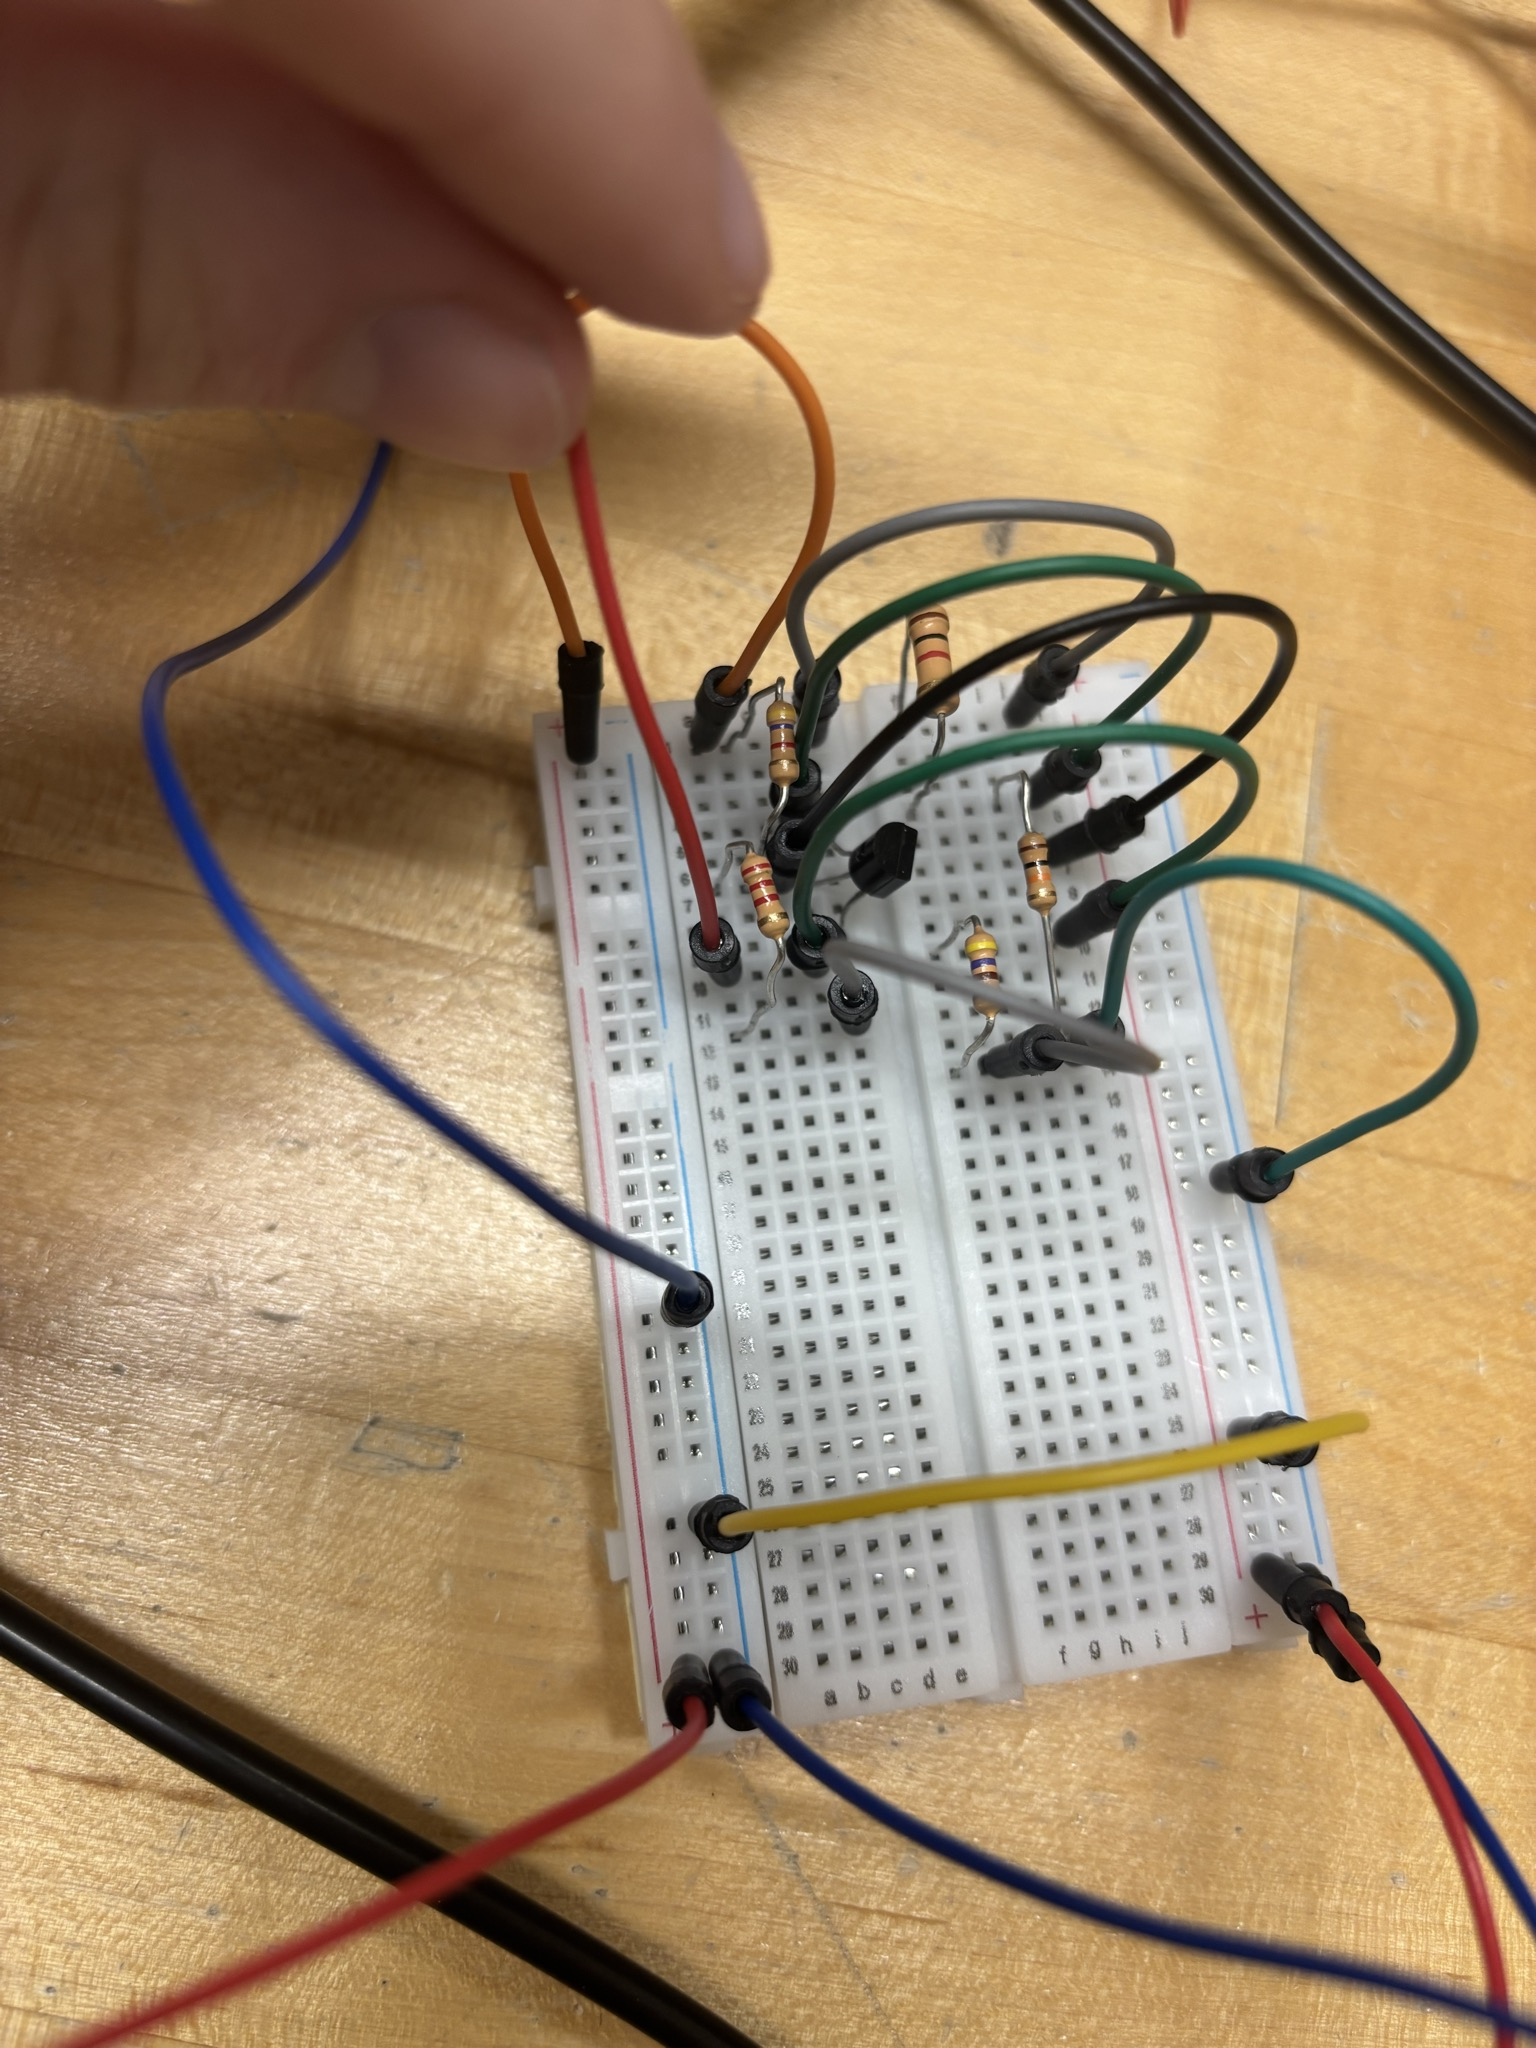
\includegraphics[width=0.5\textwidth]{assets/c1.jpeg }
	\caption{Transistor Circuit Implementation}
	\label{fig:hw}
\end{figure}

The circuit was implemented on a breadboard. The left - column was
short-circuited to the right + column to form the ground. 5 volt voltage
differences were applied across both the left and right +/- columns. The base
pin of the transistor is connected to row 6 of the left half, along with the
4.7 $k\Omega$ and 2.2 $k\Omega$ resistors. The collector pin is wired to row 4
of the right half, along with the 1 $k\Omega$ and 10 $k\Omega$ resistors. The
emitter pin is wired to row 10 of the right half, along the with 470 $\Omega$
resistor. The red and blue wires in the upper area of the circuit were used for
taking measurements; they have no bearing on the circuit's effects. The
measured voltages are given in Table \ref{tab:hw-res}.

\begin{table}[H]
	\center
	\caption{Hardware Implementation Results}
	\begin{tabular}{|c|c|c|c|c|}
		\hline
		        & V$_\text{B}$ & V$_\text{C}$ & V$_\text{E}$ & V$_\text{BE}$ \\
		\hline
		\hline
		Results & -1.851 V     & -0.624 V     & -2.549 V     & 0.697 V       \\
		\hline
		Error   & 0.7\%        & 5.2\%        & 0.5\%        & 0.4\%         \\
		\hline
	\end{tabular}
	\label{tab:hw-res}
\end{table}

As seen in Table \ref{tab:hw-res}, the only measurement with significant error
was that of V$_\text{C}$. Every hardware measurement is within a three
hundreths of a volt of simulated values; however, because the voltatge is much
smaller at V$_\text{C}$, percent error is greatly increased. Nonetheless, a
5\% error is reasonable.

\section{Conclusion}

All results are given in Table \ref{tab:res}.

\begin{table}[H]
	\center
	\caption{Final Lab Results}
	\begin{tabular}{|c|c|c|c|c|}
		\hline
		           & V$_\text{B}$ & V$_\text{C}$ & V$_\text{E}$ & V$_\text{BE}$ \\
		\hline
		\hline
		Hand calc  & −1.837 V     & −0.658 V     & −2.537 V     & 0.700 V       \\
		\hline
		Simulation & -1.838 V     & -0.658 V     & -2.537 V     & 0.700 V       \\
		\hline
		Hardware   & -1.851 V     & -0.624 V     & -2.549 V     & 0.697 V       \\
		\hline
	\end{tabular}
	\label{tab:res}
\end{table}

Transistors are common and useful circuit components. The work done in this
laboratory demonstrated how to analyze their circuits and voltages for use in
future projects. There were no issues in the calculation, simulation, or
implementation of the circuit. All measured values were within reasonable
ranges of their simulated and calculated counterparts. The exercise was
successful.

\section{Acknowledgements}

Methods described in the textbook \textit{Fundamentals of Electric Circuits,
	7th Ediition} \cite{fec} were used to derive node voltages for Figure
\ref{fig:c1}.

The CircuiTi$k$Z \cite{ctz} manual was consulted in the creation in Figure
\ref{fig:c1}.

The template for this Technical Memo was modified from a \LaTeX \ class created
by Joshua Milas and Seth Gower, using the provided Tech Memo Template and
example Tech Memo from the Advanced Course as inspiration.

The Teaching Assistant, Sol Holston, verified that calculated, simulated, and
measured values were correct.

\printbibliography

\end{document}
